\documentclass{article}
\iffalse
This file is protected by Copyright. Please refer to the COPYRIGHT file
distributed with this source distribution.

This file is part of OpenCPI <http://www.opencpi.org>

OpenCPI is free software: you can redistribute it and/or modify it under the
terms of the GNU Lesser General Public License as published by the Free Software
Foundation, either version 3 of the License, or (at your option) any later
version.

OpenCPI is distributed in the hope that it will be useful, but WITHOUT ANY
WARRANTY; without even the implied warranty of MERCHANTABILITY or FITNESS FOR A
PARTICULAR PURPOSE. See the GNU Lesser General Public License for more details.

You should have received a copy of the GNU Lesser General Public License along
with this program. If not, see <http://www.gnu.org/licenses/>.
\fi
\author{} % Force author to be blank
%----------------------------------------------------------------------------------------
% Paper size, orientation and margins
%----------------------------------------------------------------------------------------
\usepackage{geometry}
\geometry{
	letterpaper,			% paper type
	portrait,				% text direction
	left=.75in,				% left margin
	top=.75in,				% top margin
	right=.75in,			% right margin
	bottom=.75in			% bottom margin
 }
%----------------------------------------------------------------------------------------
% Header/Footer
%----------------------------------------------------------------------------------------
\usepackage{fancyhdr} \pagestyle{fancy} % required for fancy headers
\renewcommand{\headrulewidth}{0.5pt}
\renewcommand{\footrulewidth}{0.5pt}
\rhead{\small{ANGRYVIPER Team}}
%----------------------------------------------------------------------------------------
% Appendix packages
%----------------------------------------------------------------------------------------
\usepackage[toc,page]{appendix}
%----------------------------------------------------------------------------------------
% Defined Commands & Renamed Commands
%----------------------------------------------------------------------------------------
\renewcommand{\contentsname}{Table of Contents}
\renewcommand{\listfigurename}{List of Figures}
\renewcommand{\listtablename}{List of Tables}
\newcommand{\todo}[1]{\textcolor{red}{TODO: #1}\PackageWarning{TODO:}{#1}} % To do notes
\newcommand{\code}[1]{\texttt{#1}} % For inline code snippet or command line
%----------------------------------------------------------------------------------------
% Various pacakges
%----------------------------------------------------------------------------------------
\usepackage{hyperref} % for linking urls and lists
\usepackage{graphicx} % for including pictures by file
\usepackage{listings} % for coding language styles
\usepackage{rotating} % for sideways table
\usepackage{pifont}   % for sideways table
\usepackage{pdflscape} % for landscape view
%----------------------------------------------------------------------------------------
% Table packages
%----------------------------------------------------------------------------------------
\usepackage{longtable} % for long possibly multi-page tables
\usepackage{tabularx} % c=center,l=left,r=right,X=fill
\usepackage{float}
\floatstyle{plaintop}
\usepackage[tableposition=top]{caption}
\newcolumntype{P}[1]{>{\centering\arraybackslash}p{#1}}
\newcolumntype{M}[1]{>{\centering\arraybackslash}m{#1}}
%----------------------------------------------------------------------------------------
% Block Diagram / FSM Drawings
%----------------------------------------------------------------------------------------
\usepackage{tikz}
\usetikzlibrary{shapes,arrows,fit,positioning}
\usetikzlibrary{automata} % used for the fsm
%----------------------------------------------------------------------------------------
% Colors Used
%----------------------------------------------------------------------------------------
\usepackage{colortbl}
\definecolor{blue}{rgb}{.7,.8,.9}
\definecolor{ceruleanblue}{rgb}{0.16, 0.32, 0.75}
\definecolor{drkgreen}{rgb}{0,0.6,0}
\definecolor{deepmagenta}{rgb}{0.8, 0.0, 0.8}
\definecolor{cyan}{rgb}{0.0,0.6,0.6}
\definecolor{maroon}{rgb}{0.5,0,0}
%----------------------------------------------------------------------------------------
% Update the docTitle and docVersion per document
%----------------------------------------------------------------------------------------
\def\docTitle{Component Data Sheet}
\def\docVersion{1.4}
%----------------------------------------------------------------------------------------
\date{Version \docVersion} % Force date to be blank and override date with version
\title{\docTitle}
\lhead{\small{\docTitle}}

\def\comp{temp}
% do not delete this line, it is used by the auto gen script to insert latex code
\def\comp{iqstream\_max\_calculator}
%GEN_COMPLC_NAME
\def\Comp{TEMP}
% do not delete this line, it is used by the auto gen script to insert latex code
\def\Comp{Iqstream\ Max\ Calculator }
%GEN_COMPUC_NAME
\graphicspath{ {figures/} }

\def\comp{iqstream\_max\_calculator}
\edef\ecomp{iqstream_max_calculator}
\def\Comp{IQStream Max Calculator}


\begin{document}

\section*{Summary - \Comp}
\begin{tabular}{|c|M{13.5cm}|}
	\hline
	\rowcolor{blue}
	                  &                                                                                \\
	\hline
	Name              & \comp                                                                          \\
	\hline
	Worker Type       & Application                                                                    \\
	\hline
	Version           &  v\docVersion \\
	\hline
	Release Date      &  October 2018 \\
	\hline
	Component Library &  ocpi.assets.util\_comps \\
	\hline
	Workers           &  \comp.hdl, \comp.rcc \\
	\hline
	Tested Platforms  &  ml605, centos7 \\
	\hline
\end{tabular}

\section*{Functionality}
\subsection*{in/out ports}
Messages are passed directly from the \verb+in+ port to the \verb+out+ port. Backpressure is transfered to the \verb+in+ port from the \verb+out+ port.
\subsection*{max\_I\_is\_valid Property}
Indicates \verb+max_I+ is valid. Will be false if no data has
                       been received on \verb+in\verb+ port since either a) the last read of
                       \verb+max_I+ or b) the worker first went into the operating
                       state.
\subsection*{max\_Q\_is\_valid Property}
Indicates \verb+max_Q+ is valid. Will be false if no data has
                       been received on \verb+in+ port since either a) the last read of
                       \verb+max_I+ or b) the worker first went into the operating
                       state.
\subsection*{max\_I Property}
Max I value observed on \verb+in+ port. Value will be -32768
                       when worker first enters the operating state and will be
                       reset to -32768 after each read. \verb+max_I_is_valid+ should
                       always be read prior to reading this property because
                       \verb+max_I_is_valid+ will immediately be set to false once
                       \verb+max_I+ is read.
\subsection*{max\_Q Property}
Max Q value observed on \verb+in+ port. Value will be -32768
                       when worker first enters the operating state and will be
                       reset to -32768 after each read. \verb+max_Q_is_valid+ should
                       always be read prior to reading this property because
                       \verb+max_I_is_valid+ will immediately be set to false once
                       \verb+max_Q+ is read.

\section*{Worker Implementation Details}
\subsection*{\comp.hdl}
The \comp.hdl worker has \verb+IDATA_WIDTH_p+ and \verb+ODATA_WIDTH_p+ parameter properties which facilitate the build parameterization of DataWidth of the \verb+in+ and \verb+out+ ports.

\section*{Block Diagrams}
\subsection*{Top level}
\subsection*{\comp.rcc}
\begin{center}
  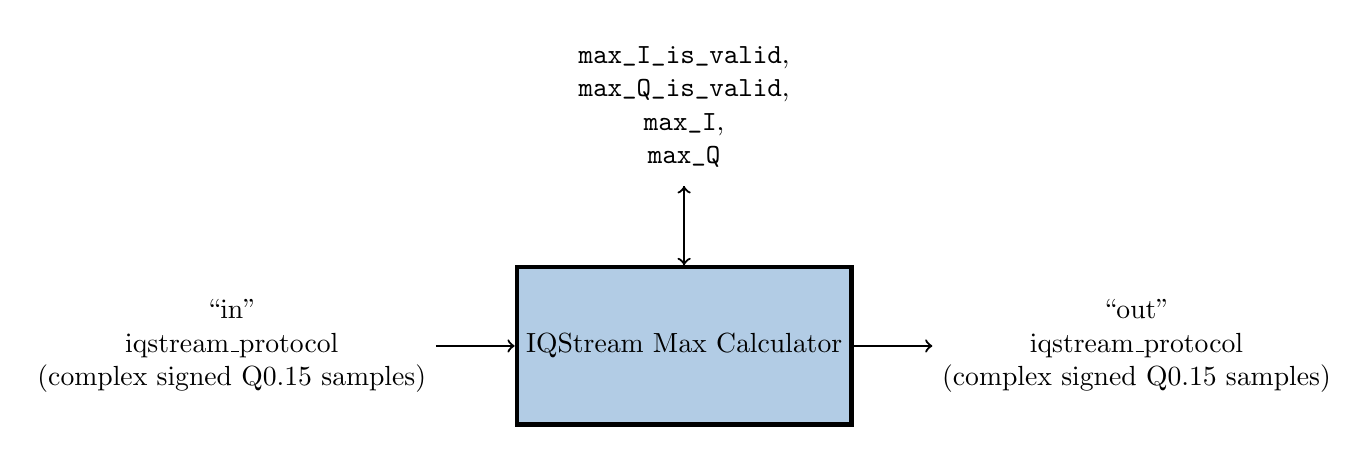
\begin{tikzpicture}[% List of styles applied to all, to override specify on a case-by-case
      every node/.style={
        align=center,     % use this so that the "\\" for line break works
        minimum size=2cm  % creates space above and below text in rectangle
      },
      every edge/.style={draw,thick}
    ]
    \node[rectangle,ultra thick,draw=black,fill=blue](R2){\Comp};
    \node[rectangle,draw=white,fill=white](R3)[left= of R2]{``in'' \\ iqstream\_protocol \\ (complex signed Q0.15 samples) };
    \node[rectangle,draw=white,fill=white](R4)[right= of R2]{``out'' \\ iqstream\_protocol \\ (complex signed Q0.15 samples) };
    \node[rectangle,draw=white,fill=white](R5)[above= of R2]{\verb+max_I_is_valid+, \\ \verb+max_Q_is_valid+, \\ \verb+max_I+, \\ \verb+max_Q+};
    \path[->]
    (R3)edge [] node [] {} (R2)
    (R2)edge [] node [] {} (R4)
    (R2)edge [] node [] {} (R5)
    (R5)edge [] node [] {} (R2)
    ;
  \end{tikzpicture}
\end{center}
\subsection*{\comp.hdl}
\begin{center}
  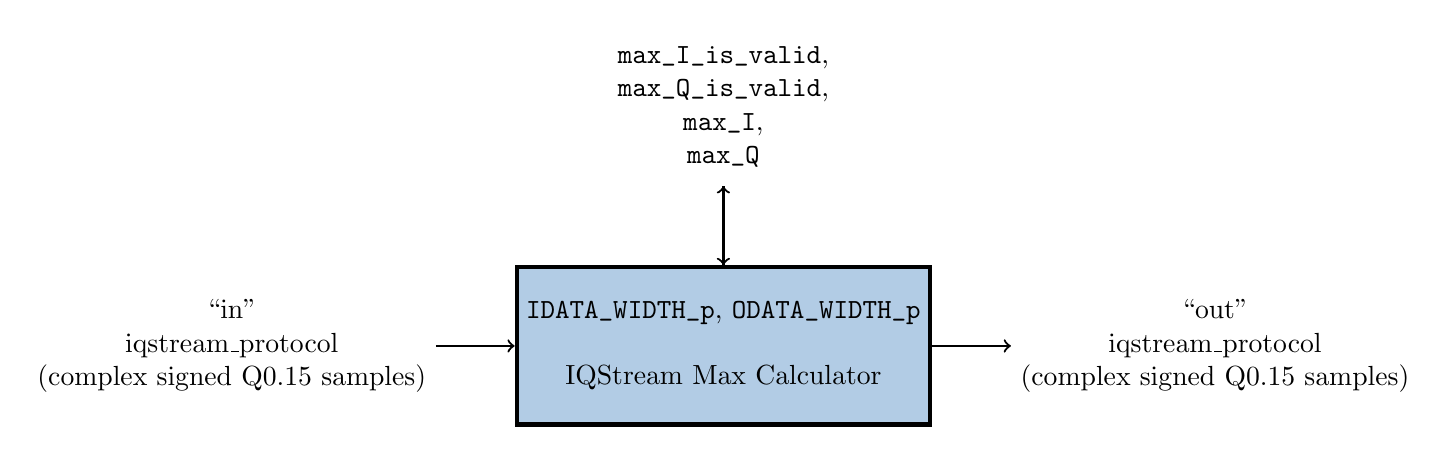
\begin{tikzpicture}[% List of styles applied to all, to override specify on a case-by-case
      every node/.style={
        align=center,     % use this so that the "\\" for line break works
        minimum size=2cm  % creates space above and below text in rectangle
      },
      every edge/.style={draw,thick}
    ]
    \node[rectangle,ultra thick,draw=black,fill=blue](R2){\verb+IDATA_WIDTH_p+, \verb+ODATA_WIDTH_p+ \\ \\ \Comp};
    \node[rectangle,draw=white,fill=white](R3)[left= of R2]{``in'' \\ iqstream\_protocol \\ (complex signed Q0.15 samples) };
    \node[rectangle,draw=white,fill=white](R4)[right= of R2]{``out'' \\ iqstream\_protocol \\ (complex signed Q0.15 samples) };
    \node[rectangle,draw=white,fill=white](R5)[above= of R2]{\verb+max_I_is_valid+, \\ \verb+max_Q_is_valid+, \\ \verb+max_I+, \\ \verb+max_Q+};
    \path[->]
    (R3)edge [] node [] {} (R2)
    (R2)edge [] node [] {} (R4)
    (R2)edge [] node [] {} (R5)
    (R5)edge [] node [] {} (R2)
    ;
  \end{tikzpicture}
\end{center}\pagebreak

\section*{Source Dependencies}
\subsection*{\comp.rcc}
assets/components/util\_comps/\comp.hdl/\comp.cc
\subsection*{\comp.hdl}
assets/components/util\_comps/\comp.hdl/\comp.vhd

\begin{landscape}
	\section*{Component Spec Properties}
	\begin{scriptsize}
% do not delete this line, it is used by the auto gen script to insert latex code
\begin{tabular}{|p{3cm}|p{1.5cm}|c|c|c|p{1.5cm}|p{1cm}|p{6cm}|}
\hline
\rowcolor{blue}
Name                 & Type   & SequenceLength & ArrayDimensions & Accessibility       & Valid Range & Default & Usage
\\
\hline
max\_I\_is\_valid & bool  & - & - & Volatile & -  &- & Indicates \verb+max_I+ is valid.
\\
\hline
max\_Q\_is\_valid & bool  & - & - & Volatile & -  &- & Indicates \verb+max_Q+ is valid.
\\
\hline
max\_I & short  & - & - & Volatile & -  &- & Max I value observed on in port.
\\
\hline
max\_Q & short  & - & - & Volatile & -  &- & Max Q value observed on in port.
\\
\hline
\end{tabular}
%GEN_SPEC_TABLE
	\end{scriptsize}

	\section*{Worker Properties}
	\subsection*{\comp.hdl}
	\begin{scriptsize}
% do not delete this line, it is used by the auto gen script to insert latex code
%GEN_WORKER_TABLE
\begin{tabular}{|p{3cm}|p{1.5cm}|c|c|c|p{1.5cm}|p{1cm}|p{6cm}|}
\hline
\rowcolor{blue}
Name                 & Type   & SequenceLength & ArrayDimensions & Accessibility       & Valid Range & Default & Usage
\\
\hline
IDATA\_WIDTH\_p & ushort & - & - & Parameter & -  & 32 & -
\\
\hline
ODATA\_WIDTH\_p & ushort & - & - & Parameter & -  & 32 & -
\\
\hline
\end{tabular}
	\subsection*{\comp.rcc}
\begin{tabular}{|p{3cm}|p{1.5cm}|c|c|c|p{1.5cm}|p{1cm}|p{5cm}|}
\hline
\rowcolor{blue}
Name                 & Type   & SequenceLength & ArrayDimensions & Accessibility       & Valid Range & Default & Usage
\\
max\_I & - & - & - & ReadSync & -  &- & -
\\
\hline
max\_Q & - & - & - & ReadSync & -  &- & -
\\
\hline
\end{tabular}
	\end{scriptsize}

	\section*{Component Ports}
	\begin{scriptsize}
% do not delete this line, it is used by the auto gen script to insert latex code
\begin{tabular}{|M{2cm}|M{1.5cm}|M{4cm}|c|c|M{9cm}|}
\hline
\rowcolor{blue}
Name & Producer & Protocol & Optional & Advanced & Usage
\\
\hline
in & false & iqstream\_protocol.xml& False & - & -\\
\hline
out & true & iqstream\_protocol.xml& true & - & -\\
\hline
\end{tabular}
%GEN_PORT_TABLE
	\end{scriptsize}

	\section*{Worker Interfaces}
	\subsection*{\comp.hdl}
	\begin{scriptsize}
\begin{tabular}{|M{2cm}|M{1.5cm}|M{4cm}|c|M{12cm}|}
\hline
\rowcolor{blue}
Type & Name & DataWidth & Advanced & Usage
\\
\hline
StreamInterface & in & \verb+IDATA_WIDTH_p+ & - & -\\
\hline
StreamInterface & out & \verb+ODATA_WIDTH_p+ & - & -\\
\hline
\end{tabular}
%GEN_INTERFACE_TABLE
	\end{scriptsize}
\end{landscape}

\section*{Control Timing and Signals}
\subsection*{\comp.hdl}
\begin{flushleft}
Data is passed from the input port to the output port with the minimum possible latency. In the absence of backpressure, this latency is one clock cycle. Note that, in the absence of backpressure, all input ports have a latency of one clock cycle.
\end{flushleft}

\begin{landscape}
\section*{Worker Configuration Parameters}
\subsubsection*{\comp.hdl}
\input{../../\ecomp.hdl/configurations.inc}
\section*{Performance and Resource Utilization}
\subsubsection*{\comp.rcc}
\subsubsection*{\comp.hdl}
\input{../../\ecomp.hdl/utilization.inc}
\end{landscape}


\section*{Test and Verification}
\begin{flushleft}
No unit test for this component exists. However, a hardware-in-the-loop
application (which is NOT a unit test) exists for testing purposes (see
assets/applications/iqstream\_max\_calculator\_test).
\end{flushleft}
\end{document}
